\documentclass{university}

\course{هوش مصنوعی}
\subject{تمرین سوم بخش دوم}
\professor{دکتر رهبان}

\begin{document}

\setupdocument

\section{}

\subsection{}
امید ریاضی در حالت عادی در شکل 
\ref{fig:eNormal}
آمده است.

\begin{figure}[htbp]
    \centering
    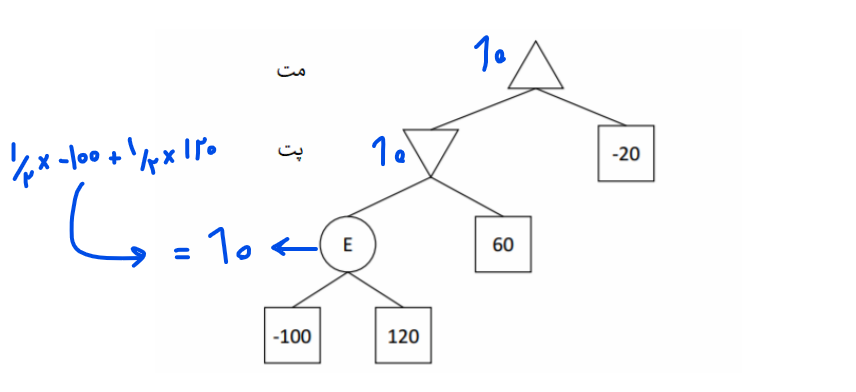
\includegraphics[width=0.8\textwidth]{assets/a.png}
    \caption{امید ریاضی در حالت عادی}
    \label{fig:eNormal}
\end{figure}

\subsection{}
هر دو حالت در شکل‌های 
\ref{fig:eOneHundredTwenty}
و
\ref{fig:minusOneHundred}
نشان داده شده‌اند. 

\begin{figure}[htbp]
    \centering
    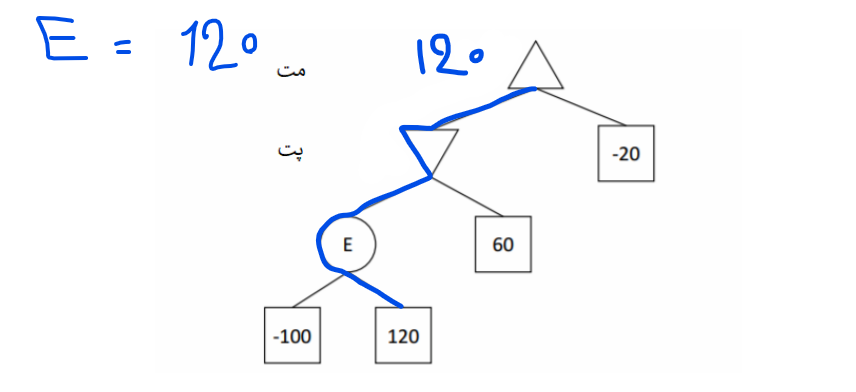
\includegraphics[width=0.8\textwidth]{assets/b120.png}
    \caption{امید ریاضی در حالت تقلب مت و مقدار 120}
    \label{fig:eOneHundredTwenty}
\end{figure}
\begin{figure}[htbp]
    \centering
    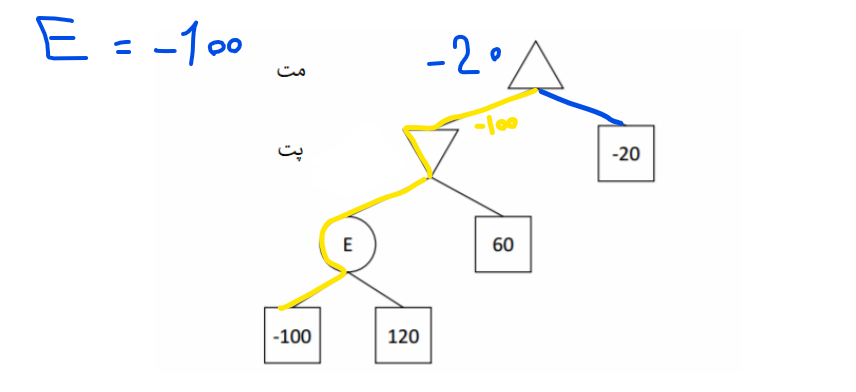
\includegraphics[width=0.8\textwidth]{assets/b-100.png}
    \caption{امید ریاضی در حالت تقلب مت و مقدار منفی 100}
    \label{fig:minusOneHundred}
\end{figure}

\subsection{}
به طور میانگین امید ریاضی پولی که مت بدست می‌آورد 40 واحد افزایش داشته.
$$
\frac{-20 + 120}{2} - 10 = 40
$$

\subsection{}
هر دو حالت در شکل‌های 
\ref{fig:eOneHundredTwentyBoth}
و
\ref{fig:minusOneHundredBoth}
نشان داده شده‌اند. 

\begin{figure}[htbp]
    \centering
    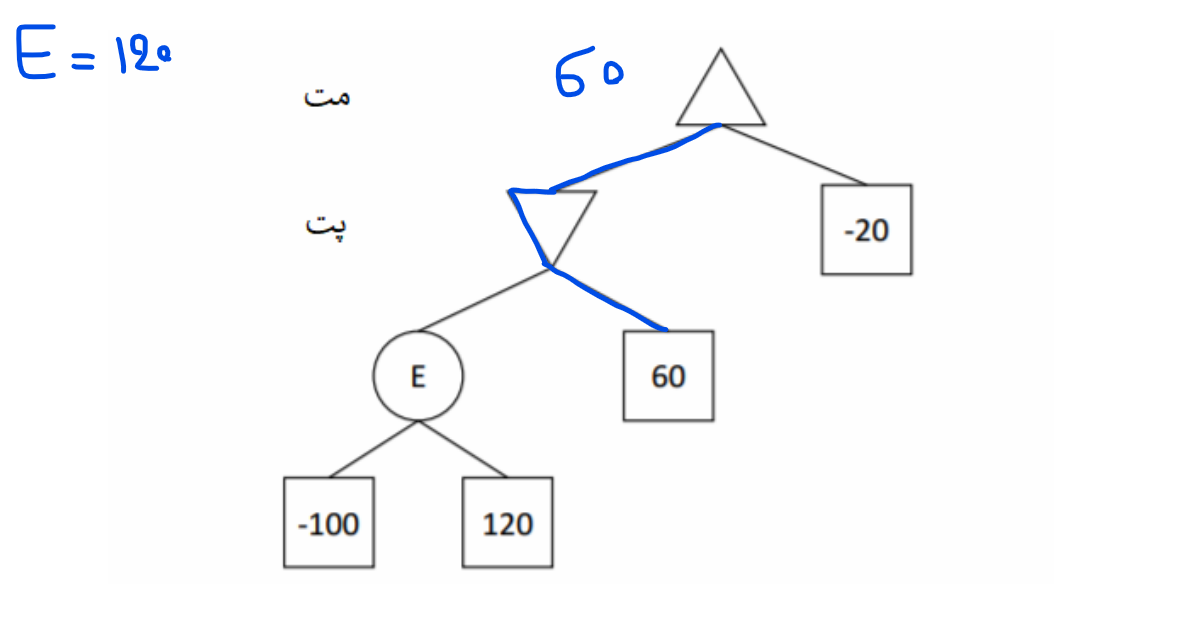
\includegraphics[width=0.8\textwidth]{assets/c120.png}
    \caption{امید ریاضی در حالت تقلب هردو و مقدار 120}
    \label{fig:eOneHundredTwentyBoth}
\end{figure}
\begin{figure}[htbp]
    \centering
    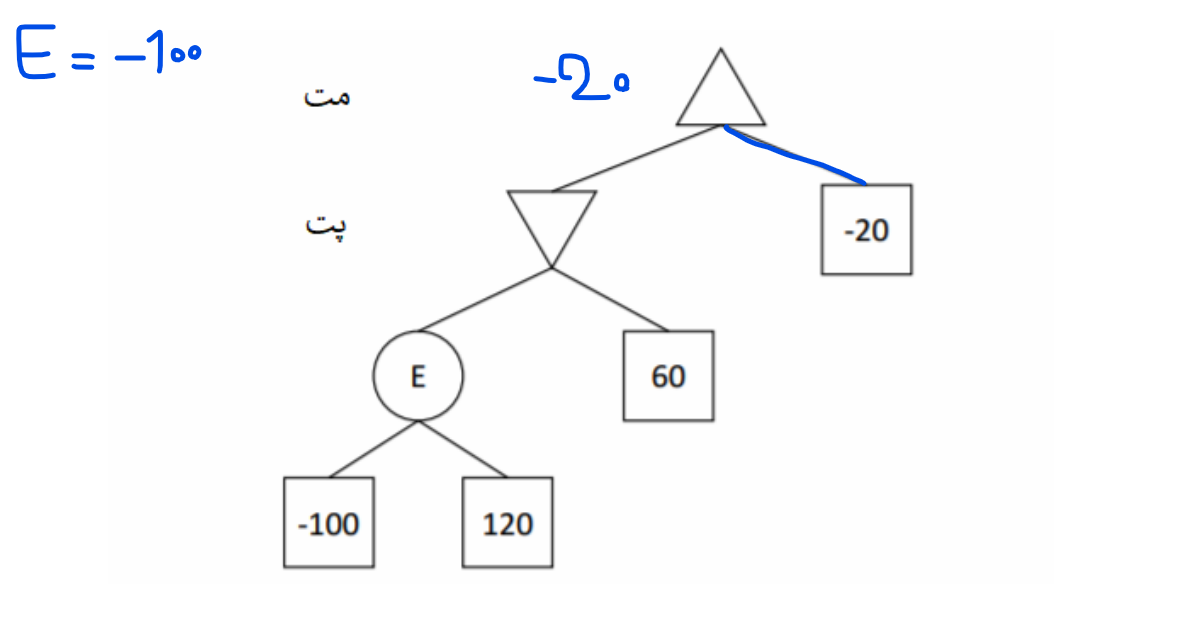
\includegraphics[width=0.8\textwidth]{assets/c-100.png}
    \caption{امید ریاضی در حالت تقلب هردو و مقدار منفی 100}
    \label{fig:minusOneHundredBoth}
\end{figure}

\subsection{}
در حالتی که هیچ یک تقلب نکنند، امید ریاضی پول بدست آمده 
\lr{$10$}
است. 

در حالتی که هر دو تقلب کنند، امید ریاضی پول بدست آمده به صورت میانگنین
\lr{$20$}
است.
$$
\frac{60 + (-20)}{2} = 20
$$

پس در حالتی که هردو تقلب کنند به نفع مت است. این منطقی است چون مت اول انتخاب می‌کند.
و در بازی سالم و بدون تقلب به نفع پت است.

\end{document}